%% Related Work
%%=========================================

\chapter{Related Work}
\label{ch:related_work}
This chapter presented related work that can lay the foundation for our system. Basing our system on the task of translation, we look closer at natural language processing, specifically recent work in the area of machine translation. Establishing the state of the art in this area, we present the underlying work that make up these systems by explaining their architecture and implementation.

%%=========================================

\section{Natural Language Processing}
\label{sec:natural_language_processing}
In 1954, a translation system developed at Georgetown University was demonstrated for the first time. The system did fully automatic translation of more than sixty sentences from Russian to English. One of the creators, Léon Dostert, predicted that automatic text-reading translations machines would be finished within three to five years \citep{hutchins1997first}. As research continued, the complexity of the linguistic problems became more and more apparent. Critics argued that the concept of fully automatic high quality translations that could produce translations indistinguishable from those of humans translators were impossible in principle \citep{hutchins2007machine}. National Science Foundation established the Automatic Language Processing Advisory Committee (ALPAC) in 1964, to carry out a study of the realities of machine translation. In 1966 they published their report that concluded that the use of machine translation was slower, less accurate and twice as expensive as human translation. The report also said that there was no immediate or predictable prospect of useful machine translation \citep{hutchins2007machine, national1966language, koehn2010statistical}. The ALPAC report led to a decrease of research in the area, but it did not stop completely.

It was first as the later half of the 1970s and the early 1980s that machine translation again saw a rise in popularity. The latter half of the 1980s also saw a general revival in interest in interlingua systems. This interest was motivated in part by artificial intelligence, which was also a research field that attracted much attention. Since the 1980s, new methods such as corpus-based approaches and statistical machine translation based systems. Speech translation has also seen growing interest since the late 1980s \citep{hutchins2007machine}.

\begin{figure}[H]
    \centering
    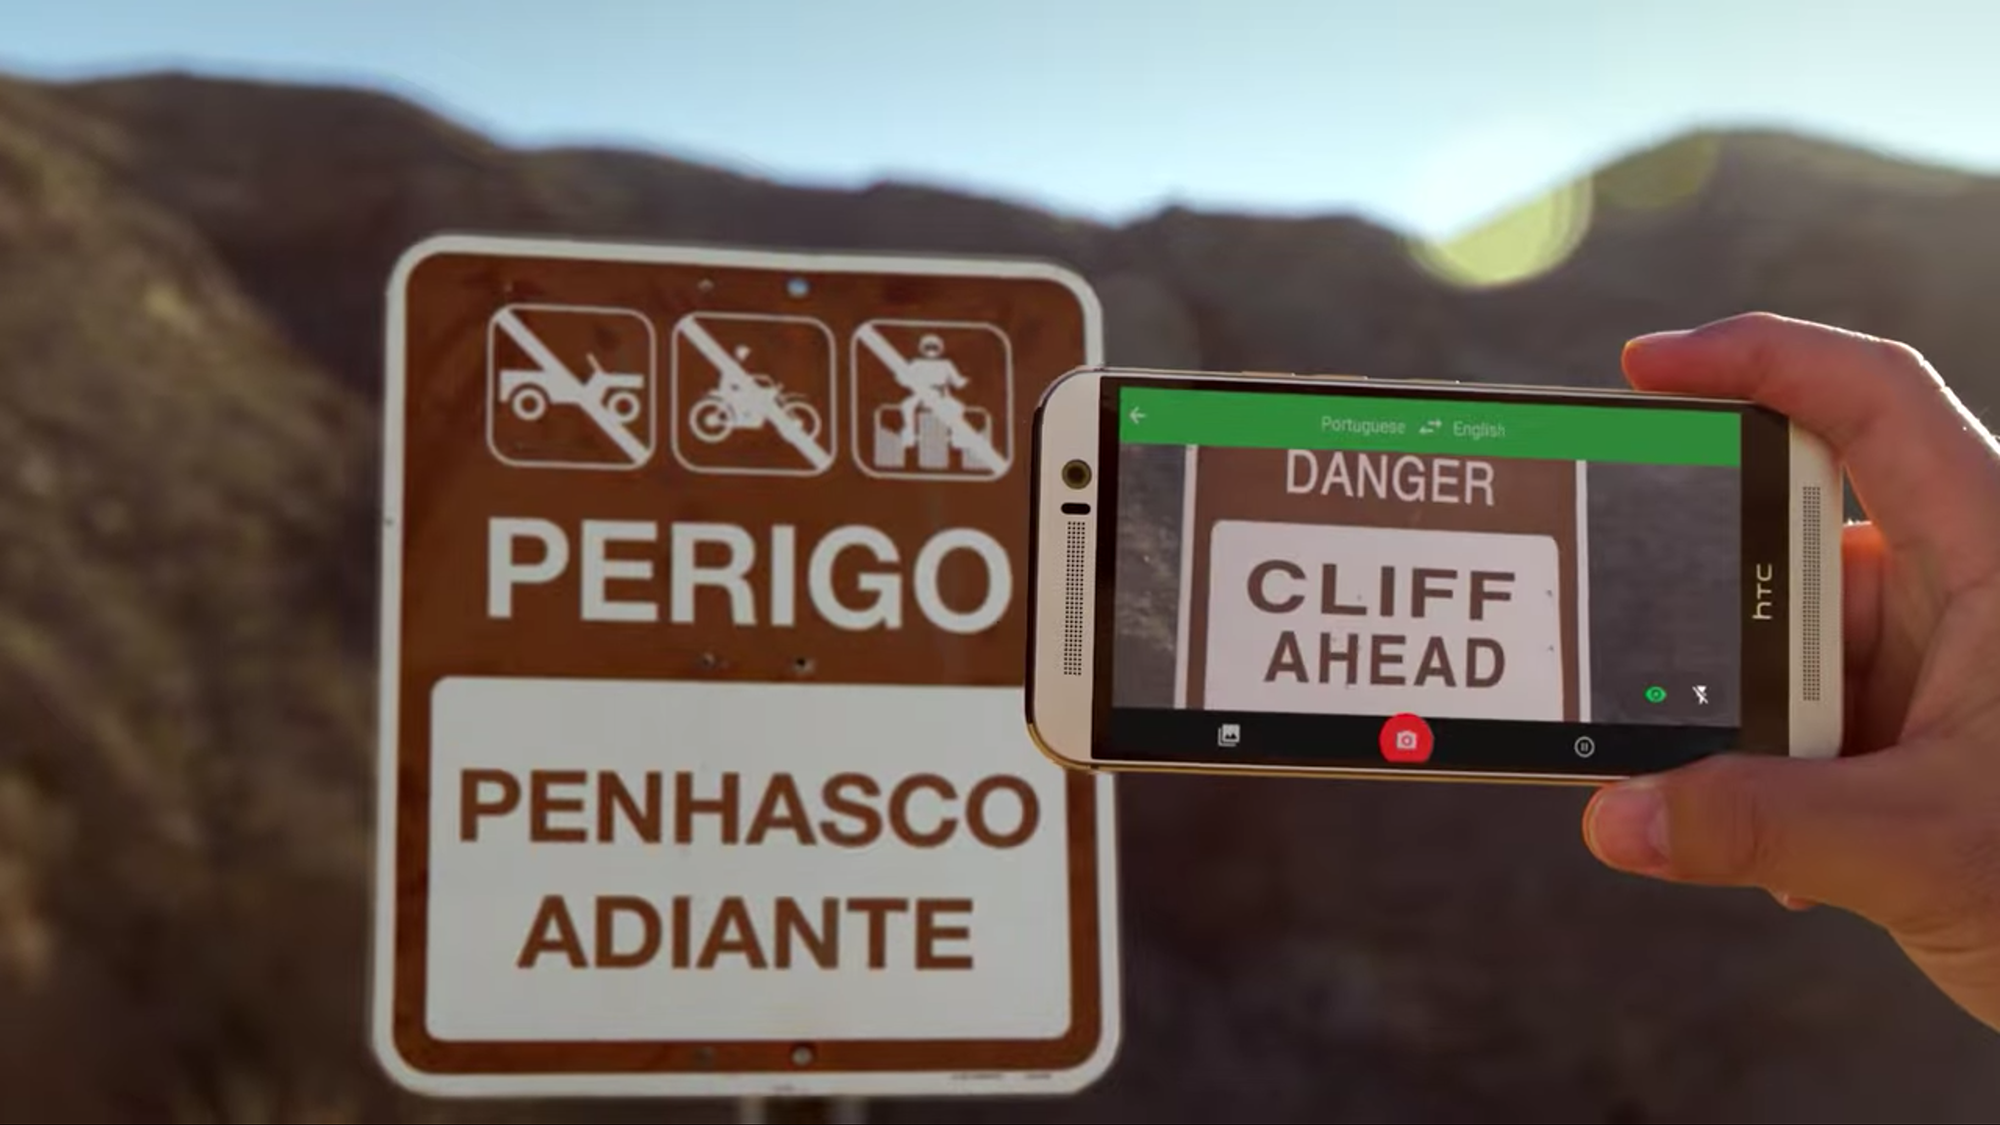
\includegraphics[width=0.7\textwidth]{fig/background_theory/google_translate_rt.png}
    \caption{The Google Translate app and its image translation feature}
    \label{fig:google-translate-rt}
\end{figure}

In recent years, online solution such as Google Translate\footnote{https://translate.google.com} and AltaVista's Babelfish\footnote{https://www.babelfish.com} has gained much popularity. Both services offers on-demand translation for free \citep{hutchins2007machine}. Google reported on their blog in 2016 that their service now supported over 100 languages, had more than 500 million users and translated more than 100 billion words a day \citep{turovsky2016googletranslate}. The native app for Google Translate has also become very popular. It offers the same functionality as their online counterpart, but also offer a few additional features, such as ``Word Lens" which translates images in place.

%%=========================================

\section{Statistical Machine Translation}
\begin{figure}[ht]
    \centering
    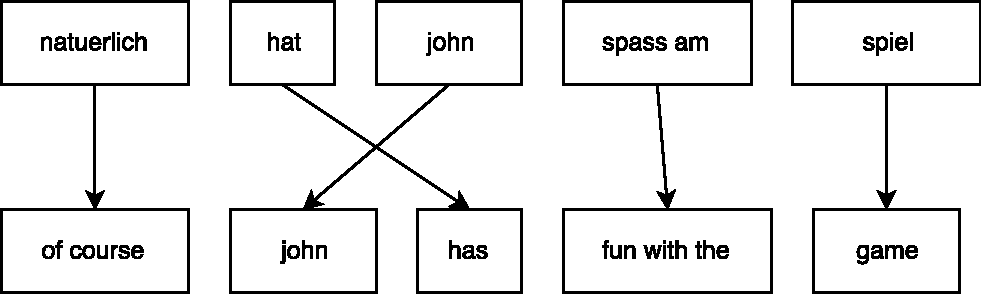
\includegraphics[width=0.7\textwidth]{fig/related_work/translation_de_en.pdf}
    \caption{Phrase-based translation of a German sentence to English}
    \label{fig:translation-phrase-based}
\end{figure}

For the past two decades or so, machine translation has taken a new direction. Instead of pre-defined rule-based systems, many modern machine translation systems attack the problem of machine translation with statistical methods and ideas from information theory \citep{brown1990statistical}. Statistical machine translation was born as an idea in the 1980s in the labs of IBM Research. The idea came in the wake of success of statistical methods in speech recognition. The idea was to model the translation task as a statistical optimization problem. Some of the best performing SMT systems today are phrase-based, an approach where the input sequence is broken up into a sequence of phrases, and these phrases are mapped one-to-one to output phrases, which may be reordered \citep{koehn2010statistical}. See Figure \ref{fig:translation-phrase-based} for illustration of a phrase-based translation of a German sentence to English.

Statistical machine translation has been the dominant translation paradigm for decades \citep{wu2016google}. Variants and implementations of SMT based systems have achieved state of the art performance in machine translation \citep{watanabe07onlinelargemargin}. There now also exists SMT systems on the commercial market, a market long dominated by the well-established rule-based methods \citep{hutchins2007machine}.

%%=========================================

\section{Neural Machine Translation}
Neural machine translation is another approach to machine translation that has emerged recently. This approach aims at building a jointly-tuned single neural network which is trained to maximize translation performance. This is a different approach from traditional statistical machine translation systems, where a translation system consists of sub components that are optimized separately \citep{wolk2015neural}. The great benefit of neural machine translation systems is its ability to learn directly, in an end-to-end fashion. 

In 2016, Google published their work on Google's Neural Machine Translation system, or GNMT for short. This system replaced their older statistical machine translation system that ran Google Translate \citep{turovsky2016googletranslatenmt}. GNMT uses the common sequence-to-sequence learning framework as proposed by \citep{sutskever2014sequence, wu2016google}. This framework uses multilayered Long Short-Term Memory (LSTM) to map the input sequence to a vector of a fixed dimensionality, and then another LSTM to decode the target sequence from the fixed vector. Their implementation is closely related to the work of \citep{kalchbrenner2013recurrent} who were the first to map the input sentence into a vector, and then back into a sentence. It also build heavily on the neural network architecture presented by \citep{cho2014learning}. They did this using LSTM-like RNN architecture, although their primary focus was to integrate their neural network into an SMT system \citep{cho2014learning, sutskever2014sequence}. The work of \citep{sutskever2014sequence} did the entire translation end-to-end and was not integrated with any other frameworks or systems. Their implementation achieved close-to-best results in an English to French translation task, and outperformed various SMT-based systems.

\begin{figure}[ht]
    \centering
    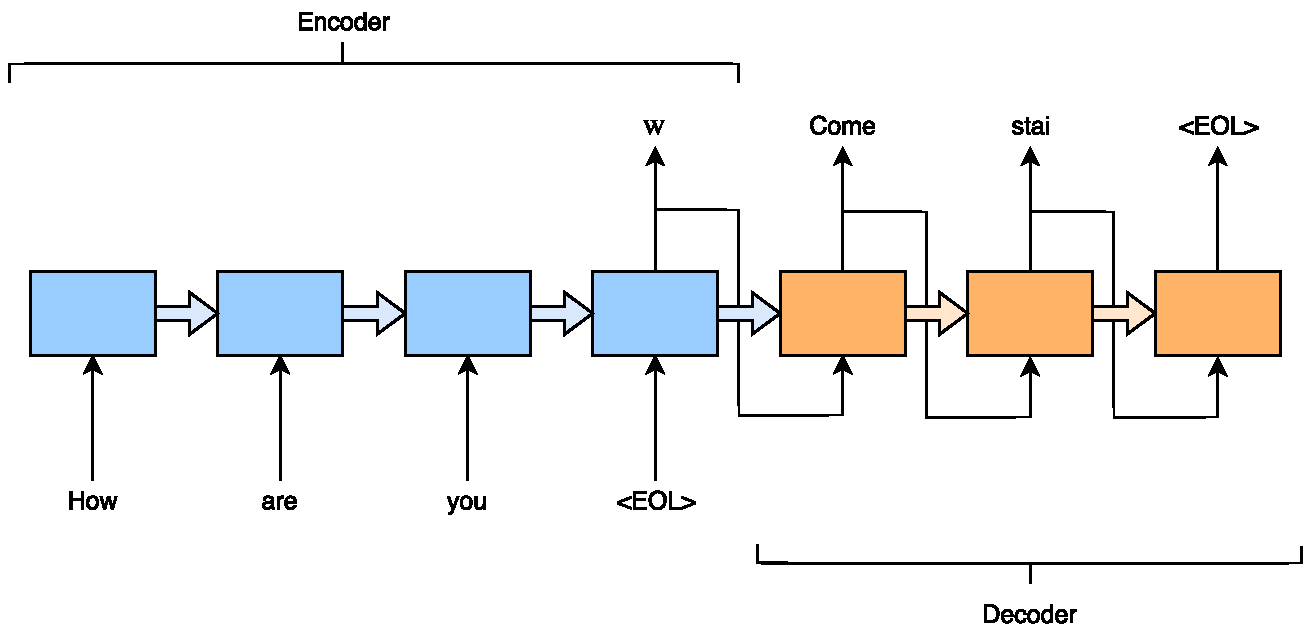
\includegraphics[width=0.8\textwidth]{fig/related_work/encoder_decoder_en_it.pdf}
    \caption{General translation approach in neural machine translation from an English sentence to Italian}
    \label{fig:machine-translation-encoder-decoder-simple}
\end{figure}

The encoder-decoder approach, as further explained in section \ref{sec:encoder-decoder}, has also been used as the foundation for various other NMT architectures. \citep{chung2016character} used the encoder-decoder general approach in their experiment, although they used bi-scale recurrent network with gated recurrent units (GRU), instead of LSTMs. They showed that their model, which did translation on a sequence of characters, without any explicit word segmentation, using a charachter-level decoder, could outperform the one with a subword-level decoder.

\citep{bahdanau2014neural} proposed another model, which did not use the fixed-length vector that the encoder produces. They argued that the fixed-length vector was a bottleneck in improving the performance of the encoder-decoder approach. Their argument was that the neural network needed to compress all the necessary information of a source sentence into a fixed-length vector, which may make make it difficult to cope with longer sentences. This was already shown in the analysis by \citep{cho2014properties}, where a variant of \citep{cho2014learning} as well as a novel network dubbed \textit{gated recursive convolutional neural network} were evaluated. Their evaluation showed that both architectures performed relatively well on short sentences, but suffered significantly as the length of the sentences increased. The model proposed by \citep{bahdanau2014neural} instead learns to align and translate joinly. It does this by encoding the input sequence into a sequence of vectors and chooses a subset of these vectors adaptively while decoding the translation. This model outperformed the basic encoder-decoder significantly in their experiments.

\iffalse
\begin{itemize}
    \item Talk fast about ``ORDER MATTERS: SEQUENCE TO SEQUENCE FOR SETS"
    \item Talk about ``Addressing the Rare Word Problem in Neural Machine Translation", this can be in greater detail
    \item At some point talk about something that also uses attention. Needs to present this too.
\end{itemize}
\fi

%%=========================================

\section{Neural Network}
At the base of the neural machine translation systems are neural networks. The idea of models using artificial neurons, can be traced back to the 1940s. Since then, more sophisticated proposals and variants have been made from decade to decade. Artificial neural networks are an attempt at modeling the information process capabilities of nervous systems, found in the brain. This is done by implementing mathematical models of neurons \citep{russell2010aimodernapproach}.

\begin{figure}[ht]
    \centering
    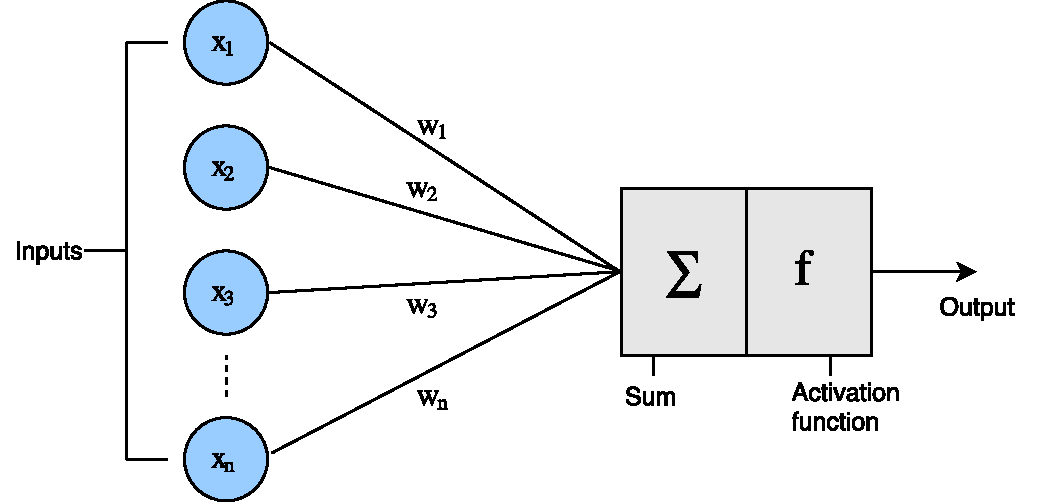
\includegraphics[width=0.8\textwidth]{fig/related_work/nn_perceptron.pdf}
    \caption{Illustration of a mathematical model of a neuron}
    \label{fig:nn-perceptron}
\end{figure}

Figure \ref{fig:nn-rnn} illustrates a simple mathematical model for a neuron, often called a unit or a node. This unit ``fires" when a linear combination of its inputs exceeds some threshold. A neural network is a collection of many such units. The properties of a network is determined by its topology, as well as the properties of the units. Networks are constructed by directly linking nodes with each other. A link from unit \(i\) to unit \(j\) serves to propagate the activation \(a_{i}\) from \(i\) to \(j\). The strength and sign of the signal is determined by the numeric weight that is associated with the unit. A feed-forward network consists of units which has connections that only goes in one direction. These node receives input from the ``upstream" nodes, and delivers output to the ``downstream" nodes, forming a directed acyclic graph \citep{russell2010aimodernapproach}.

\subsection{Recurrent Neural Network}
Another way to construct a neural network is by using loops. A recurrent neural network \citep{rumelhart1988learning} is a network much like a feed-forward network, but in addition to feeding ``downstream" nodes, nodes also feeds its output back into its own inputs. This type of architecture can support a short-term memory, a feature that is necessary in problems where input also depends on previous input \citep{russell2010aimodernapproach}. For example would such characteristics be necessary if we fed the network words in a sentence, and we asked the network to predict the next word it had not yet seen. 

\begin{figure}[ht]
    \centering
    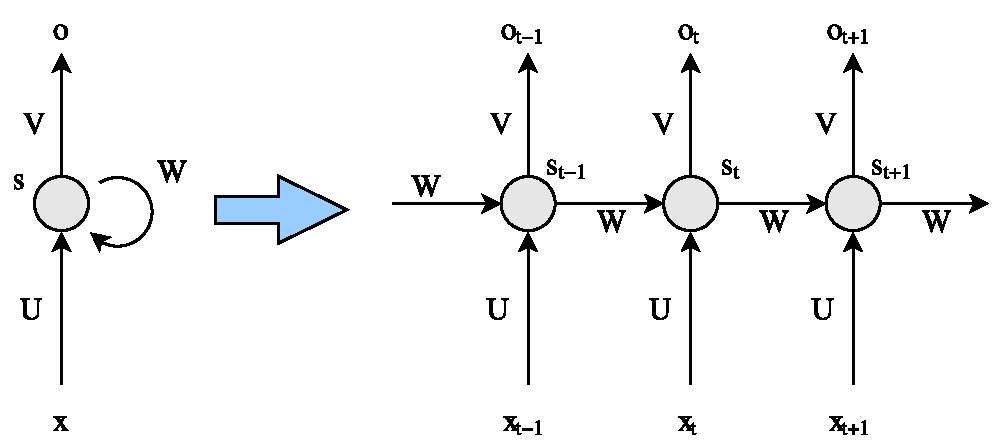
\includegraphics[width=0.7\textwidth]{fig/related_work/nn_recurrent.pdf}
    \caption{A compact and an unfolded recurrent neural network}
    \label{fig:nn-rnn}
\end{figure}

We can consider RNNs as a type of loop, and we can also unfold it into a complete sequence, as illustrated in Figure \ref{fig:nn-rnn}. In the figure, \(x_{t}\) is the input, and \(s_{t}\) is the hidden state of the recurrent network at time step \(t\). The hidden state functions as its memory as it is reused in the next time step, along with the input of the current time step. It is also important to note that the network shares the same weights \(W\) across several time steps.The recurrent neural network has input to hidden connections parametrized by a weight matrix \(U\), as well as hidden-to-hidden recurrent connections parametrized by a weight matrix \(W\). In addition, the network has hidden-to-output connection parametrized by a weight matrix \(V\) \citep{goodfellow2016deeplearning}.

\begin{align}
    \begin{split}\label{eq:rnn-eq-1}
        h_{t}&=\sigma(b+Ws_{t-1}+Ux_{t})
    \end{split}\\
    \begin{split}\label{eq:rnn-eq-2}
        \hat{y_{t}}&=\sigma(c+Vh_{t})
    \end{split}
\end{align}

Equations \ref{eq:rnn-eq-1} and \ref{eq:rnn-eq-2} are slightly modified from \citep{goodfellow2016deeplearning}, and defines the forward propagation of the model illustrated in Figure \ref{fig:nn-rnn}. The parameters \(b\) and \(c\) are the bias vectors. Computing the gradient in a recurrent neural network is done with a back-propagation algorithm called back-propagation through time \citep{werbos1990backpropagation}. 

\subsection{Long-Short Term Memory}
The Long-Short Term Memory (LSTM) is a recurrent neural network architecture. It was first purposed by \citep{hochreiter1997long}, and was meant to address some of the shortcomings of more basic recurrent neural network architectures. \citep{bengio1994learning} showed that recurrent neural network faced an increasingly difficult problem as the duration of the dependencies to be captures increases. While the architecture could take into account short-term dependencies rather well, long-term dependencies were increasingly difficult to learn. The LSTMs were explicitly designed to avoid the long-term dependency problem. 

\begin{figure}[ht]
    \centering
    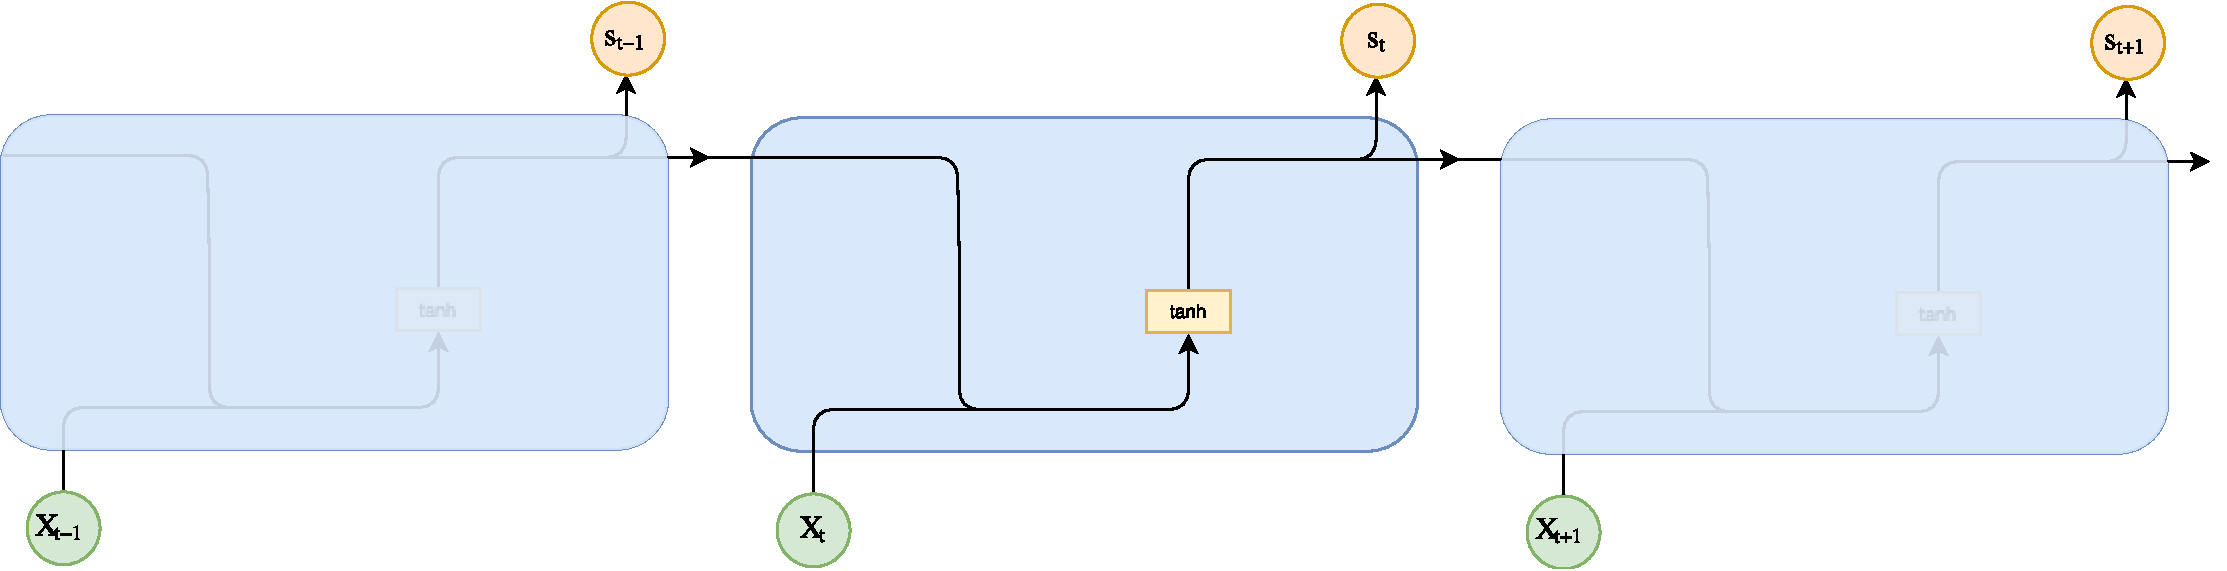
\includegraphics[width=1\textwidth]{fig/related_work/rnn_flow.pdf}
    \caption{Flow of a standard RNN}
    \label{fig:nn-rnn-flow}
\end{figure}

Figure \ref{fig:nn-rnn-flow} illustrates the chain like structure of standard recurrent neural network. Its architecture is relatively simple, containing only one layer. In this illustration our layer uses the hyperbolic tangent function (tanh).

\begin{figure}[ht]
    \centering
    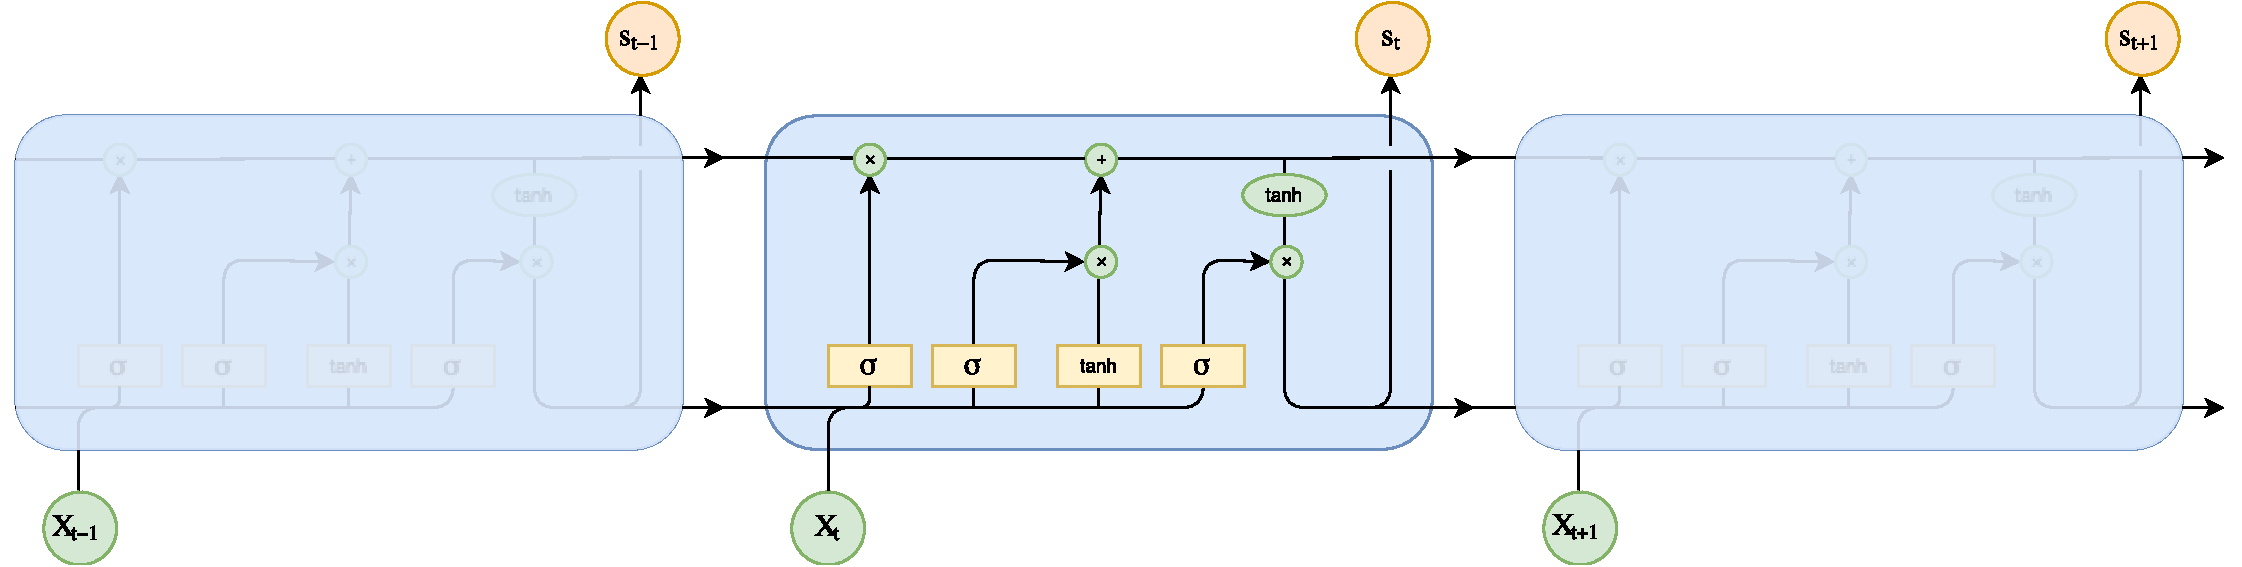
\includegraphics[width=1\textwidth]{fig/related_work/lstm_flow.pdf}
    \caption{Flow of a LSTM cell}
    \label{fig:nn-lstm-flow}
\end{figure}

Figure \ref{fig:nn-lstm-flow} illustrates a similar chain structure, but that of a LSTM cell. The LSTM module has a different structure, and instead of having a single neural network layer, like the simpler RNN, it has four layers. The topmost horizontal line carries the cell state of the unit. The LSTM unit is enriched by several co-called gating units. These gates regulate what information is remembered by the cell state, and what is forgotten. The leftmost sigmoid layer is called the ``forget gate layer". This gate decides what the state should forgotten from the existing information. The next sigmoid gate is called the ``input gate layer" and determines which values should be updated. The hyperbolic tangent gate layer creates a vector of candidate values, which could be added to the cell state. After the state is updated, or the candidate is thrown away, the final sigmoid gate, the ``output gate layer" decides what the parts of the cell state should be outputted \citep{hochreiter1997long, goodfellow2016deeplearning, olah2015lstm}.

%%=========================================

\section{Encoder-Decoder}
\label{sec:encoder-decoder}

The encoder-decoder framework is centralized around two recurrent neural networks. The idea is to encode the input in the first neual network, and decode it in the second network. The first neural network, also called the encoder, reads the input sentence, a sequence of vectors \(X = (x_{1}, x_{2}, ..., x_{n})\). This sequence is then encoded into a vector \(c\), which may or may not be of fixed length.

\iffalse
\section{Notes}


Since sequence-to-sequence models were proposed for machine translation (Sutskever et al., 2014; Cho et al., 2014; Kalchbrenner & Blunsom, 2013), the research community has proposed several applications in which these models can perform mappings from and/or to sequences. For example, image captioning maps from an image to a sentence (Vinyals et al., 2015c; Mao et al., 2015; Donahue et al., 2015), parsing maps from a sentence to a (linearized) parse tree (Vinyals et al., 2015b)

Amazing results:
Within three years of invention, outperforming models
developed over the past 15 years, and deployed in
commercial systems
- Incredibly simple implementation:
Traditional machine translation (e.g. 6k lines of Python)
Neural machine translation (e.g. 280 lines of Python)
- Machine translation as machine learning:
Easy to apply new machine techniques directly

http://www.cs.cmu.edu/~tbergkir/11711fa16/neubig16afnlp.pdf

\subsection{Other things}
Statistical machine translation (SMT) is a machine translation paradigm where translations are generated on the basis of statistical models whose parameters are derived from the analysis of bilingual text corpora. The statistical approach contrasts with the rule-based approaches to machine translation as well as with example-based machine translation. - https://en.wikipedia.org/wiki/Statistical\_machine\_translation



\subsection{5346}
Deep Neural Networks (DNNs) are powerful models that have achieved excel- lent performance on difficult learning tasks. Although DNNs work well whenever large labeled training sets are available, they cannot be used to map sequences to sequences. (5346)

Almost better than the current state of the art. SMT syste (?) research this. 5346.

5346, reuse cite 13, 7, DNNs good results on speech recognition.

Despite their flexibility and power, DNNs can only be applied to problems whose inputs and targets can be sensibly encoded with vectors of fixed dimensionality. It is a significant limitation, since many important problems are best expressed with sequences whose lengths are not known a-priori. For example, speech recognition and machine translation are sequential problems. Likewise, ques- tion answering can also be seen as mapping a sequence of words representing the question to a sequence of words representing the answer. It is therefore clear that a domain-independent method that learns to map sequences to sequences would be useful. 5346

There have been a number of related attempts to address the general sequence to sequence learning problem with neural networks. Our approach is closely related to Kalchbrenner and Blunsom [18] who were the first to map the entire input sentence to vector, and is very similar to Cho et al. [5]. Graves [10] introduced a novel differentiable attention mechanism that allows neural networks to focus on different parts of their input, and an elegant variant of this idea was successfully applied to machine translation by Bahdanau et al. [2]. The Connectionist Sequence Classification is another popular technique for mapping sequences to sequences with neural networks, although it assumes a monotonic alignment between the inputs and the outputs [11]. 5346

Third, we found it extremely valuable to reverse the order of the words of the input sentence. So for example, instead of mapping the sentence a,b,c to the sentence $\alpha, \beta, \gamma$, the LSTM is asked to map c,b,a to $\alpha, \beta, \gamma$, where $\alpha, \beta, \gamma$ is the translation of a, b, c. This way, a is in close proximity to $\alpha$, b is fairly close to $\beta$, and so on, a fact that makes it easy for SGD to “establish communication” between the input and the output. We found this simple data transformation to greatly boost the performance of the LSTM.

%%=========================================

\section{Recurrent Neural Network}
Sequence to sequence type problems have been solve

Traditional neural networks assume and inputs and outputs are independent on each other. While this is true for some problems, for other problems there is a direct connection between earlier input and following output. Recurrent Neural Networks were designed around this relationship.

Recurrent Neural Networks, or RNNs, are a class of artificial neural networks with special characteristics. Due to how RNNs have their connections between the units, it is capable of storing an internal state for the network. This state can be used to ``remember" previous outputs and computations. This makes it possible to evaluate input on the basis of previous knowledge and apply this to the output. Recurrent in Recurrent Neural Networks, means that the calculating task is done recurrent for the input.

\red{Figure here}

Because RNNs have a concept of memory and time, it is able to use previous input and feed the knowledge from that back into its internal state. 

\subsection{Use of RNNs}
\red{TODO}

%%=========================================

\section{Variations of RNNs}
\red{TODO}

\subsection{Long Short Term Memory}
Long Short Term Memory, or LSTM for short, is a method that improves on storing information over extended time in recurrent networks. 

Recurrent does, 

\cite{hochreiter1997long}

\subsection{GRU}
\red{TODO}

%%=========================================

\section{Encoder/Decoder}
\red{TODO}

\cite{rocktaschel2015reasoning}
\fi